%%%%%%%%%%%%%%%%%%%%%%%%%%%%
% CHAPTER 7 - DISCUSSION UXP
%%%%%%%%%%%%%%%%%%%%%%%%%%%%
%%%%%%%%%%%%%%%%%%%%%%%%%%%%%%%%%%%%%%%%%%%%%%%%%%%%%%%%%%%%%%%%%%%%%%%%%%%%%%%%%%%%%%%%%%
% Richard Boardman PhD Thesis: Improving Tool Support for Personal Information Management
%%%%%%%%%%%%%%%%%%%%%%%%%%%%%%%%%%%%%%%%%%%%%%%%%%%%%%%%%%%%%%%%%%%%%%%%%%%%%%%%%%%%%%%%%%

%%%%%%%%%%%%%%%%%%%%%%%%%%%%%%%%%%%%%%%%%%%%%%%%%%%%%%%%%%%%%%%%%%%%%%%%%%%%%%%%%%%%%%%%%%
% NATBIB NOTES
%%%%%%%%%%%%%%%%%%%
%\citet{jon90}                ->    Jones et al. (1990) 
%   \citet[chap.~2]{jon90}       ->    Jones et al. (1990, chap. 2)
%   \citep{jon90}                ->    (Jones et al., 1990) 
%   \citep[chap.~2]{jon90}       ->    (Jones et al., 1990, chap. 2) 
%%%%%%%%%%%%%%%%%%%%%%%%%%%%%%%%%%%%%%%%%%%%%%%%%%%%%%%%%%%%%%%%%%%%%%%%%%%%%%%%%%%%%%%%%%
\newpage
%%%%%%%%%%%%%%%%%%%%%%%%%%%%%%%%%%%%%%%%%%%%%%%%%%%%
\section{PIM User Experience}
\label{discussion:uxp}
%%%%%%%%%%%%%%%%%%%%%%%%%%%%%%%%%%%%%%%%%%%%%%%%%%%%

% This section discusses PIM user experience. 
% A simple model is presented to explain some of the observations regarding the level of satisfaction felt by a user towards their current PIM strategies as reflected in their level of organization. 
% \textbf{Section~\ref{discussion:theoretical-framework}} discussed PIM from three theoretical perspectives: as a supporting activity (\textbf{Section~\ref{discussion:supporting}}), as a cross-tool activity (\textbf{Section~\ref{discussion:cross-tool}}), and as an ongoing activity (\textbf{Section~\ref{discussion:ongoing}}).  This section builds on the second and third of these perspectives to develop a model of \textit{long-term user experience} regarding PIM, as reflected in changes in PIM strategy over time.  This based on the change data from \textbf{Chapter~\ref{chapter:main-study}}.
% INTRO: \textbf{Section~\ref{discussion:methodological-discussion}} highlighted the lack of evaluation metrics appropriate for evaluating PIM interfaces.  This section considers the concept of user experience with respect to PIM.  Based on the results from the studies reported in this thesis, a number of possible qualitative evaluation measures are proposed.

%%%%%%%%%%%%%%%%%%%%%%%%%%%%%%%%%%%%%%%%%%%%%%%%%%%%%%%%%%%%%%%%%%%%%%%%%%%%%%%%%%%%%%%%%%%%%%%%%%%%%%%%%%%%%%%%%
%%%%%%%%%%%%%%%%%%%%%%%%%%%%%%%%%%%%%%%%%%%%%%%%%%%%%%%%%%%%%%%%%%%%%%%%%%%%%%%%%%%%%%%%%%%%%%%%%%%%%%%%%%%%%%%%%
%%%%%%%%%%%%%%%%%%%%%%%%%%%%%%%%%%%%%%%%%%%%%%%%%%%%%%%%%%%%%%%%%%%%%%%%%%%%%%%%%%%%%%%%%%%%%%%%%%%%%%%%%%%%%%%%%
%%%%%%%%%%%%%%%%%%%%%%%%%%%%%%%%%%%%%%%%%%%%%%%%%%%%%%%%%%%%%%%%%%%%%%%%%%%%%%%%%%%%%%%%%%%%%%%%%%%%%%%%%%%%%%%%%

%%%%%%%%%%%%%%%%%%%%%%%%%%%%%%%
% \subsection{PIM user experience}
%%%%%%%%%%%%%%%%%%%%%%%%%%%%%%%

%%%%%%%%%%%%%%%%%%%%%%%%%%%%%%%%%%%%%%%%%%%%%%%%
% \subsection{PIM user experience}
%%%%%%%%%%%%%%%%%%%%%%%%%%%%%%%%%%%%%%%%%%%%%%%%
% \label{discussion:uxp-intro}
% Develop ideas on user experience and incorporate ideas from the previous section.
%%%%%%%%%%%%%%%%%%%%%%%%%%%%%%%%%%%%%%%%%%%%%%%%%%%%

% LIMITATIONS OF TRAD MEASURES: 
Traditional measures of usability focus on performance-related metrics of efficiency, accuracy and productivity~\citep{ad:01,preece:02}.  Preece et al. describe a recent shift towards a wider set of design goals related to the concept of \textit{user experience} -- ``what the use of a system feels like to the user''.  They discuss a series of experience-related design goals such as enjoyability and motivation which are hard to assess with traditional measures.  Similarly, \citet{ad:01} argues the importance of user-experience in evaluating designs.  In particular, he highlights the inadequacy of traditional usability measures for many high-level, ongoing tasks such as information retrieval and data analysis.  Dillon notes that in such tasks, efficiency may not be the user's priority.  Furthermore, such tasks do not always have a definite goal, meaning that effectiveness may be hard to define.
% \textit{Also talk about Dillon who urges a focus on satisfaction over efficiency and effectiveness.}  \textit{Focus here on investigating indicators of satisfaction or user experience.}
The author observes that Dillon's arguments also apply to PIM.  \textbf{Section~\ref{exp-study:Results-comparison}} reported observations of ``irrational user behaviour'', such as storing items that are never used.  In such cases, participants were using interfaces in a clearly inefficient manner.  \textbf{Section~\ref{discussion:ongoing}} discussed the ongoing nature of PIM.  Although, effectiveness may be meaningful for discrete one-off PIM events (e.g. moving a folder), it is not clear how the effectiveness of PIM-tool usage can be measured in the long-term.
%%%%%%%%%%%%%%%%%%%%%%%%%%%%%%%%%%%%%%%%%%%%%%%%%%%%%
% Short term contributant of poor user experience
%%%%%%%%%%%%%%%%%%%%%%%%%%%%%%%%%%%%%%%%%%%%%%%%%%%%%
% Previous studies -- impact on self-worth.  Guilt. Why?
%  the user experience of the study participants is considered with respect to PIM.  
This section considers what measures of user experience could be applied in the context of PIM.

Much of the feedback received from the study participants in \textbf{Chapters~\ref{chapter:exploratory_study}} and \textbf{\ref{chapter:main-study}} emphasised \textit{negative user experience} in terms of PIM -- participants liked to moan.  Many complained of the short-term problems they encountered in retrieving, naming, and classifying items. %, e.g. what to do with an item when it belongs in multiple folders, the so-called dilemma of \textit{multiple classification}.  
The effect of such one-off problems may be minor and limited to short-term frustration.  However, if they reoccur, the effects may build up over time leading to negative user experience over the long-term.   %Furthermore, the supporting nature of PIM means that users rarely devote time to planning and executing changes in strategy.  It is suggested here that a lack of serious reflection on PIM, may contribute to negative user experience, by encouraging the acceptance of non-optimal strategies.  Problems may worsen in the background, e.g. as collections become more cluttered. % (PROVIDE EVIDENCE based on F4, M8?) 
The studies provided some evidence of this.  A number of participants reported feeling ashamed or guilty over the state of one or more of their collections\footnote{The reports of shame and guilt may have been exaggerated since the participants were being asked for a guided tour by the author.  However, other studies have also reported this phenomenon, e.g. ~\citep{Bellotti:00}.}.  In the extreme, such feelings may even impact a user's sense of self-worth.


% A key factor in this may be the perception that ``messy equals bad'' resulting from this social value~(Economist:03).  Current tools may exacerbate such a feeling by not auto-tidying old items, and making pro-organizing functionality highly prominent.
% \end{itemize}
%%%%%%%%%%%%%%%%%%%%%%%%%%%%%%%%%%%%
% Problems build up over the long-term
% Poor long-term user experience
%%%%%%%%%%%%%%%%%%%%%%%%%%%%%%%%%%%%
% Becomes a problem, knock-on effect on productivity. Build-up over time.	
% Problems build up over time.  Exacerbated by supporting nature of PIM.  Acceptance of non-optimal strategies by some users.
% BUILD-UP OVER TIME: 
% DESIGN IDEAS
% Do we need to move away from messy equals bad?  Do tools make it worse?
% Design questions include the question of what can be done to help certain user profiles: for example the image-concious? 



%%%%%%%%%%%
% QUESTION
%%%%%%%%%%%
% \textit{Why do some people change? Why is it hard to change?  Look at the empirical data.}
% This section considers the impact of ongoing \textit{user experience} on why people change.
% This section considers why some people encounter such negative user experience.  A simple model is proposed which attempts to explain some of the observations made in \textbf{Chapter~\ref{chapter:main-study}}.
%%%%%%%%%%%%%%%%%%%%%%%%%%%%%%%%%%%%%%%%%%%%%%%%%%%%
% LINK: Summary and connection to where this is used, what direction may be opened up}
%%%%%%%%%%%%%%%%%%%%%%%%%%%%%%%%%%%%%%%%%%%%%%%%%%%%
% METH SUGG: Impact on methodology for evaluation -- have to measure more than just efficiency.  Idea of Friedman's value-based computing. Security, robustness, to look tidy
% Measures of user experience beyond short-term costs (NB: both positive and negative user experience)

The improvement of PIM user experience should be a key concern for the designers of PIM-tools as PIM is a frequent, everyday activity. Therefore, measures of PIM user experience may be a useful qualitative evaluation metric.  A number of aspects of negative PIM user experience which could be observed in interview data are highlighted as follows:
% These considerations may offer routes for developing evaluation criteria for PIM-tools which cater for more than PIM efficiency and effectiveness.  
% Level of security in one's PIM environment may be an important indicator of user satisfaction.  
% \item control Satisfaction-related values of , ``information safety'' may be as important as the time taken to find an item:

\begin{itemize}

%%%%%%%%%%%%%%%%%%%%%%%%
% A: DO TOO LITTLE PIM
%%%%%%%%%%%%%%%%%%%%%%%%
% Do too little PIM (``little'' is subjective taking factors such as personality into account for a specific user), 
% and production activities suffer.  Too little time is spent on PIM, user may lose more items, possibly feels bad about being messy, cue poor user experience.  % Even not backing up.
% \item DO TOO LITTLE PIM 
% Like the some of the study participants in \textbf{Chapter~\ref{chapter:exploratory_study}}, the user may also feel guilty for being messy (poor user experience). 
% (self-perceived, and ``external'') ``being tidy'', ``looking tidy to others'' clutter anxiety of order
\item \textit{Sense of untidiness} -- Constrained by a finite amount of time and attention resources, the user is faced with a dilemma of how much time to spend managing information.  If the user devotes relatively little attention towards PIM, the possible consequences are that they will feel messy or worry that others will see them that way.  The user may also be concerned that their productivity may be impacted if they are unable to find items.  However, the reasons for feeling untidy may be irrational from an efficiency perspective.  For example, having a ``messy'' inbox may not impact user productivity if search is used effectively.  Whether grounded in productivity concerns or not, guilt over messiness still has the potential to cause poor user-experience.  \citet{levy:01} describes such symptoms as ``anxiety of order''. This may be expressed in terms of the user ``feeling untidy'' or ``out of control''.  Such feelings may be exacerbated by the pressure from society to see tidiness as a positive trait~\citep{Economist:03}. % Because PIM is an everyday activity, users feeling this way are continuously faced with the state of their workspace. 

% : ``everyone thinks I'm messy''. % \textit{Such guilt may even over time affect the user's self-image.}


\item \textit{Sense of wasting time} -- In contrast, guilt may also be generated if the user devotes relatively large amounts of time to PIM.  In this case, the user may feel guilty for ignoring his or her production activities.  % More time spent on PIM means less time for production activities, which may also lead to guilt.

%%%%%%%%%%%%%%%%%%%%%%%%%%%%%%
% Do too much PIM (as above), 
%%%%%%%%%%%%%%%%%%%%%%%%%%%%%%
% and production activities suffer.  Too much time is spent on PIM -- a supporting activity -- distracting the user from what they are meant to be doing.
% \item Do too much PIM: 

\end{itemize}

Each of these aspects of negative user experience, may cause the user to feel dissatisfied with their current strategies, and want to adjust them.   Several examples of ``dissatisfaction with current PIM strategies'' are provided in the next section, grounded in observations from the main study.

% Therefore, ``satisfaction with current PIM strategies'', may be a useful indicator of ongoing PIM user experience, as discussed in the following section.




% LINK TO NEXT SECTION: 

%%%%%%%%%%%%%%%%%%%%%%%%%%%%%%%%%%%%%%%%%%%%%%%%%%%%%%%%%%%%%%%%%%%%%%%%%%%%%%%%%%%%%%%%%%%%%%%%%%%%%%%%
%%%%%%%%%%%%%%%%%%%%%%%%%%%%%%%%%%%%%%%%%%%%%%%%%%%%%%%%%%%%%%%%%%%%%%%%%%%%%%%%%%%%%%%%%%%%%%%%%%%%%%%%

%%%%%%%%%%%%%%%%%%%%%%%%%%%%%%%%%%%%%%%%%%%%%%
% BEHAVIOUR either changing or unchanging
%%%%%%%%%%%%%%%%%%%%%%%%%%%%%%%%%%%%%%%%%%%%%%
%%%%%%%%%%%%%%%%%%%%%%%%%%%%%%%%%%%%%%%%%%%%%%%%
\subsection{Satisfaction with Current PIM Strategies}
%%%%%%%%%%%%%%%%%%%%%%%%%%%%%%%%%%%%%%%%%%%%%%%%
\label{discussion:uxp-settled}

%%%%%%%%%%%%%%%%%%%%%%%%%%%%%%%
% CHANGERS AND NON-CHANGERS
%%%%%%%%%%%%%%%%%%%%%%%%%%%%%%%
% People changed (incrementally) or they didn't.
During the main study reported in \textbf{Chapter~\ref{chapter:main-study}},  two types of user were identified, \textit{changers} and \textit{non-changers}, based on whether they changed strategy over the course of the study.  % \textbf{Section~\ref{main-study:discussion:changes-model}} noted that the observed changes consisted of incremental shifts in the relative proportions of information organized with specific low-level strategies.
% ATTITUDE either settled or unstable
% This section considers why some participants changed strategy, and some did not.  And attempts to discuss how ``settledness with current strategies'' can be used as a measure of user experience.
Two participants (F3 and M5) made minor changes to how certain types of information were organized.  The remaining six participants did not make significant changes to their PIM strategies. However, several of these \textit{non-changers} were dissatisfied with their strategies, and expressed the desire to change them in some way.  However, the changes they desired were often seen to be too expensive in terms of time and effort.  

Based on this analysis, two more user types are identified, based on whether users were satisfied with their current strategies.

%%%%%%%%%%%%%%%%%%%%%%%%%%%%%%%%%%%%%%%%%%
% USE IN THEORY DEV: SETTLED/UNSETTLED): 
%%%%%%%%%%%%%%%%%%%%%%%%%%%%%%%%%%%%%%%%%%
% Regarding major shifts in strategy: two user types could be identified based on how content they were with their current set of strategies: settled and unsettled.
\begin{enumerate}
\item \textit{Satisfied with current strategies} -- These users are content with their current management strategies, and do not want to change them. % and are not got down by them on an ongoing basis.

\item \textit{Dissatisfied with current strategies} -- These users are not content with their management strategies, and want to change them in some way.  % However, they may not make the changes due to the perceived costs involved.  % Therefore they may experience this sense of dissatisfaction over the long-term. %  have to live with the dissatisfaction, causing long-term negative user experience.  \textit{This may be a useful indicator of poor user experience.}

% TWO DESIRES: This leads to a desire to: (1) change tool, and (2) change practice.

\end{enumerate}


 

% Changes in strategy are related to user experience
% Propose PIM strategy personalities (stable/unstable-self-punishing)
% It is argued that users who are more unhappy with their strategy and want to change have a worse user experience. 
% there was not a direct correlation between level of organizing and whether users were settled in their strategies.
\textbf{Figure~\ref{fig:discussion:settled-unsettled-model}} presents a series of user profiles which illustrate some examples of ``strategy dissatisfaction''. These are also used to describe observations from the main study in \textbf{Chapter~\ref{chapter:main-study}}.  The horizontal axis indicates whether the user's current organizing behaviour is pro-organizing or organizing-neutral. The vertical axis indicates how satisfied the user feels towards their current strategies.  Note that the figure does not specify a particular tool context.  Five user profiles are identified as follows:
\begin{enumerate}

\item \textit{Profile A: Satisfied and organizing-neutral} -- Profile A has a pragmatic attitude towards PIM.  She considers organization to be low priority, and feels confident that she can find information when she needs it.  % She sees no benefit in filing more information and has ``better things to do''. 
Participant M7 in the main study was an example of this profile in all tool contexts -- he was satisfied with his organizing-neutral strategies and enjoyed positive user experience.
% User A is untidy and could not care less. She has a laid back attitude to clutter

\item \textit{Profile B: Satisfied and pro-organizing} -- Profile B is also satisfied, but is highly organized. She spends a lot of time filing information and believes the time and effort is worth it.  Participants M1, M2, and M6 in the main study were examples of this profile in terms of their file and email practices.  M5 is also considered an example of this profile in files and email.  Although he made pro-organizing changes to his strategies, these were relatively minor.

The remaining three profiles are examples of users who are dissatisfied with their current strategies and consequently suffering poor user experience.

\item \textit{Profile C: Dissatisfied and organizing-neutral} -- Profile C is ``image-concious''.  He considers himself untidy, and feels guilty for not being more organized.  Participant M3 was an example of this profile in his file collection: he devoted relatively little effort to organizing, but talked of the social pressure he faced to be more organized.  He made some pro-organizing changes towards the end of the study.

\item \textit{Profile D: Dissatisfied and pro-organizing}:  Like profile C, profile D is also ``image-concious''.  Although relatively organized, she is still not satisfied with the state of her workspace. Participants M4 and M8 fit this profile in terms of their file management: they both devoted a significant amount of effort to PIM, but wanted to be more organized.  However, both stated that they did not have enough time to perform the significant reorganizing they felt was necessary.  

\item	\textit{Profile E: Dissatisfied and pro-organizing} -- This last profile is a hypothetical example.  None of the study participants matched the profile, however it is included as an interesting example of behaviour.  Profile E devotes significant effort to PIM, but resents the amount of time she spends filing information, seeing it as a waste of time.  She believes that she could benefit by not filing, and instead rely on search like one of her colleagues. However, she is not willing to take the plunge and stop relying on folders.  

\end{enumerate}

%\item pragmatic
%\item image-conscious. Image-concious, ``tidy'' has become a value imposed by society. 

%%%%%%%%%%%%%%%%%%%%%%%%%%%%%%%%%%%%%%
% %%%%%%%%%%%%%%%%%%%%%%%%%%%%%%%%%%%%
% FIGURE - Settled PIM and unsettled PIM
% %%%%%%%%%%%%%%%%%%%%%%%%%%%%%%%%%%%%
%%%%%%%%%%%%%%%%%%%%%%%%%%%%%%%%%%%%%%
\begin{figure}[t]
	\begin{center}
		\leavevmode
		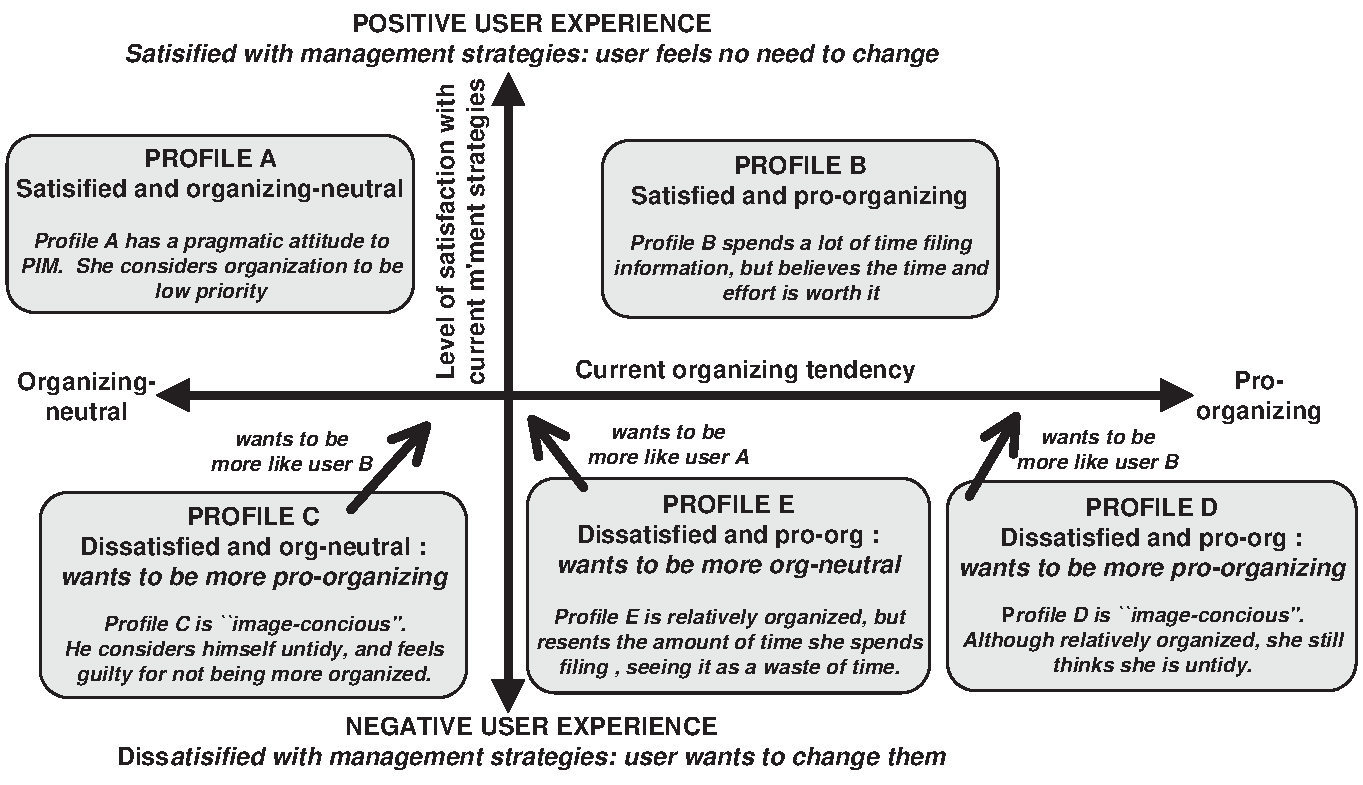
\includegraphics[width=\textwidth]{pictures/discussion/settled-unsettled-model.pdf}
	\end{center}
	\caption{Examples of poor PIM user experience caused by ``dissatisfaction with PIM strategies''}
	\label{fig:discussion:settled-unsettled-model}
\end{figure}

% There may even by a conflict between the two attitudes (organizing-neutral and pro-organizing) for some users.  For example, a user caught between profiles D and E can be envisaged although none was encountered in the process of this research. 
%%%%%%%%%%%%%%%%%%%%%%%%%%%%%%%%%%%%%%%%%%%%%%%%%%%%%%%%%%%%%%%%%%%%%%%%%%%%
% provide examples of both from both pro-org and org-neut perspectives
% The main study provided examples of both settled and unsettled users. 
%%%%%%%%%%%%%%%%%%%%%%%%%%%%%%%%%%%%%%%%%%%%%%%%%%%%%%%%%%%%%%%%%%%%%%%%%%%%
%%%%%%%%%%%%%%%%%%%%%%%%%%%%%%%%%%%%%%%%%%%%%%%%%%%%%%%%%%%%%%%%%%%%%%%%%%%%%%%%%%%%%
%Settled users (examples) of various (high-level) organizing dispositions (pro-org and org-neut), and wanting to shift both ways:
%\begin{itemize}
%	\item Settled and pro-org: M1, M2, M6
%	\item Settled and org-neut: M5, M7
%\end{itemize}
%%%%%%%%%%%%%%%%%%%%%%%%%%%%%%%%%%%%%%%%%%%%%%%%%%%%%%%%%%%%%%%%%%%%%%%%%%%%%%%%%%%%%
%Unsettled users (examples) of both pro-org and org-neut, and wanting to shift both ways:
%\begin{itemize}
%	\item Unsettled, pro-org and wanting to be more pro-org: M4, M8 (mild)
%	\item Unsettled, org-neut and wanting to be more pro-org: M3
%	\item Can one envisage unsettled, pro-org and wanting to be org-neut (yes, if aware wasting lots of time on PIM?)
%\end{itemize}
%%%%%%%%%%%%%%%%%%%%%%%%%%%%%%%%%%%%%%%%%%%%%%%%%%%%%%%%%%%%%%%%%%%%%%%%%%%%%%%%%%%%%
These examples illustrate that users with either pro-organizing or organizing-neutral behaviour may feel dissatisfied with their strategies, and want to change them in some way.  It is hypothesized that an ongoing need to change one's behaviour, combined with an inability to achieve the change, may contribute to poor PIM user experience.  This may be exacerbated if the symptoms which make the user want to perform the change get worse in the meantime.

% In contrast, users who are broadly satisfied with their strategies -- whether organizing-neutral, or pro-organizing -- will not . % THINK: look at what M6 said again
% with their level of balance/their strategies. The author therefore proposes ``satisfaction with management strategies'' as a measure of PIM user experience.  




%%%%%%%%%%%%%%%%%%%%%%%%%%%%%%%%%%%%%%%%%%%%%%%%%%%%%%%%%%%%%%%%%%%%%%%%%%%%%%%%%%%%%%%%%%%%%%%%%%%%%%%%%%%%%%%%%
%%%%%%%%%%%%%%%%%%%%%%%%%%%%%%%%%%%%%%%%%%%%%%%%%%%%%%%%%%%%%%%%%%%%%%%%%%%%%%%%%%%%%%%%%%%%%%%%%%%%%%%%%%%%%%%%%
%%%%%%%%%%%%%%%%%%%%%%%%%%%%%%%%%%%%%%%%%%%%%%%%%%%%%%%%%%%%%%%%%%%%%%%%%%%%%%%%%%%%%%%%%%%%%%%%%%%%%%%%%%%%%%%%%
%%%%%%%%%%%%%%%%%%%%%%%%%%%%%%%%%%%%%%%%%%%%%%%%%%%%%%%%%%%%%%%%%%%%%%%%%%%%%%%%%%%%%%%%%%%%%%%%%%%%%%%%%%%%%%%%%

%%%%%%%%%%%%%%%%%%%%%%%%%%%%%%%%%%%%%%%%%%%%%%%%%%%
% \subsection{Balancing PIM with production tasks}
% \label{discussion:uxp-balance}
%%%%%%%%%%%%%%%%%%%%%%%%%%%%%%%%%%%%%%%%%%%%%%%%%%%
%%%%%%%%%%%%%%%%%%%%%%%%%%%%%%%%%%%%%%%%%%%%%%%%%%%%
% \subsection{Balance model: how much time should users spend on PIM?}
%%%%%%%%%%%%%%%%%%%%%%%%%%%%%%%%%%%%%%%%%%%%%%%%%%%%
% FOUNDATION: supporting nature of PIM, paradox of PIM
%\item \textit{THINK: is this really longitudinal?}
% The study data emphasised the supporting nature of PIM -- to support production activities. 
% A model of PIM and relationship to production activities in terms of the ``need for balance'' (user needs to do enough PIM to support his/her needs, ie. need to be ``active'')
% The supporting nature of PIM leads to a paradox in terms of how much PIM should be performed by a user in support of their production tasks.  The user is faced with a dilemma:
%This section considers the dilemma faced by many users in their PIM activity.  Constrained by a finite amount of time and attention resources, the user is faced with a dilemma of how much time to spend managing information in support of their production tasks:
%\begin{enumerate}

%%%%%%%%%%%%%%%%%%%%%%%%
% A: DO TOO LITTLE PIM
%%%%%%%%%%%%%%%%%%%%%%%%
% Do too little PIM (``little'' is subjective taking factors such as personality into account for a specific user), 
% and production activities suffer.  Too little time is spent on PIM, user may lose more items, possibly feels bad about being messy, cue poor user experience.  % Even not backing up.
%\item If the user devotes relatively little attention towards PIM, the possible consequence is that their production activities may suffer. For example spending little time organizing items, may mean that it is harder to find items in the future.  Like the some of the study participants in \textbf{Chapter~\ref{chapter:exploratory_study}}, the user may also feel guilty for being messy (poor user experience).  The net effect of such problems is that the user's productivity may be impacted.

%%%%%%%%%%%%%%%%%%%%%%%%%%%%%%
% Do too much PIM (as above), 
%%%%%%%%%%%%%%%%%%%%%%%%%%%%%%
% and production activities suffer.  Too much time is spent on PIM -- a supporting activity -- distracting the user from what they are meant to be doing.
%\item However if the user devotes relatively large amounts of time to PIM -- for example by developing a new PIM strategy -- his or her production activities may also suffer.  More time spent on PIM means less time for production tasks, especially in the short-term which the user may be more focused on.
%\end{enumerate}
%This dilemma is represented diagrammatically as the balance model in \textbf{Figure~\ref{fig:discussion:balance-model}}.

%%%%%%%%%%%%%%%%%%%%%%%%%%
% mention user quotes?
%%%%%%%%%%%%%%%%%%%%%%%%%%
% Paradox: if you don't do it, you waste time, all the time you do spent on it, you are wasting time!
% Talk about people who are happy/unhappy and how they fit into the model. 
% Relate to the need for satisficing
% different individuals would tend towards different balance points.  
% Other factors would also come into play.  \textit{How important does user consider organizing to be?}
%This theoretical model can be used as a framework to discuss the varying amounts of effort that different individuals devote to PIM.  \textbf{Chapter~\ref{chapter:exploratory_study}} introduced the terms \textit{pro-organizing} and \textit{organizing-neutral} to describe the level of importance which individuals assigned to being tidy.
% For organizing-neutral users, organising is not important and consequently they may satisfice by not organizing most items.
%Organizing-neutral users may consider even moderate time spent on PIM as a waste.  Therefore they would tend towards a satisficing strategy of only organizing a few items. For them, the balance point is shifted to the right.  % However, this study data suggests that even these users will organize some stuff. 

%However, more pro-organizing users may feel compelled to devote more time to PIM, and feel able to withstand more distraction from their production tasks. \textit{It is has observed that PIM is satisficing~\citep{barreau:95}. However PIM is not satisficing for everyone. For one person, satisficing is the perfect strategy -- they can get away cutting corners. However, for another satisficing may lead to poor user experience as they are continuously faced with this mess which they feel bad about.} % as they can cut corners, and they have to for lack of time buit 



%%%%%%%%%%%%%%%%%%%%%%%%%%%%%%%%%%%%%%
% %%%%%%%%%%%%%%%%%%%%%%%%%%%%%%%%%%%%
% FIGURE - Balancing PIM and production activities
% %%%%%%%%%%%%%%%%%%%%%%%%%%%%%%%%%%%%
%%%%%%%%%%%%%%%%%%%%%%%%%%%%%%%%%%%%%%
%\begin{figure}[t]
%	\begin{center}
%		\leavevmode
%		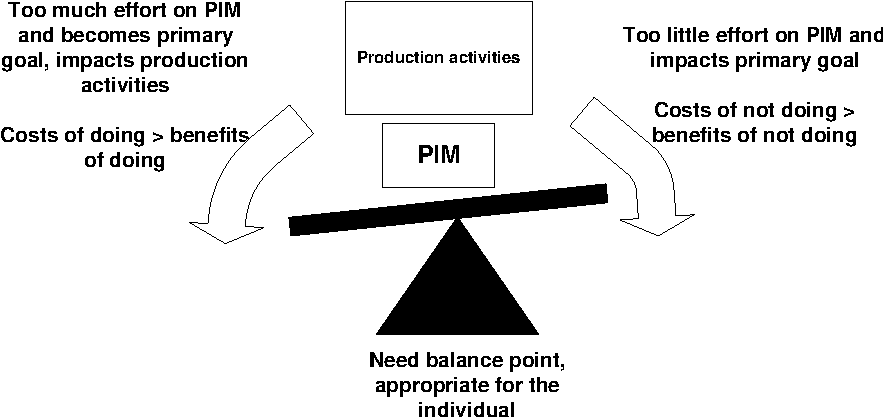
\includegraphics[width=\textwidth]{pictures/discussion/balance-model.pdf}
%	\end{center}
%	\caption{Balancing PIM and production activities}
%	\label{fig:discussion:balance-model}
%\end{figure}


%Lack of reflection (related to changes in strategy observed in main study).
% ADD: Generally people changed slowly
%Although the changes observed in the main study were subtle, participants found them beneficial.  This suggests that users may benefit from some level of reflection on PIM.  However, the supporting nature of PIM means that users rarely devote time to planning and executing changes in strategy.  It is suggested here that a lack of serious reflection on how strategies may be changed, may lead to the acceptance of non-optimal strategies.  Such problems may worsen in the background and/or get worse over time. % (PROVIDE EVIDENCE based on F4, M8?) 

%%%%%%%%%%%%%%%%%%%%%%%%%%%%%%%%%%%%%%
% TO ADD: IMPLICATIONS FOR DESIGNERS
%%%%%%%%%%%%%%%%%%%%%%%%%%%%%%%%%%%%%%
% Encouraging reflection. 
%\item As an alternative to redesigning tools to promote reflection (e.g. providing statistics on time spent filing and searching), organizations could also play a part here. Typically, organizations are more concerned with knowledge management and other strategic IT - whilst PIM is left to the individual. Nevertheless, PIM is a key aspect of employees' activities and has the potential to cause frustration and waste time. Organizations could publicize PIM-related issues, and encourage employees to self-diagnose problems to improve their PIM effectiveness. (DESIGN RECS)
%Users may benefit from increased reflection with respect to PIM, so as to receive the same benefits that resulted from the ``self-auditing'' effect of the study. As an alternative to redesigning tools to promote reflection (e.g. providing statistics on time spent filing and searching), organizations could also play a part here. Typically, organizations are more concerned with knowledge management and other strategic IT - whilst PIM is left to the individual. Nevertheless, PIM is a key aspect of employees' activities and has the potential to cause frustration and waste time. Organizations could publicize PIM-related issues, and encourage employees to self-diagnose problems to improve their PIM effectiveness.  However, managers  should take care not to be overly prescriptive, or interfere with individuals' preferred style. 
% Which of these people could benefit from increased reflection? 

%Also, the balance model proposed above raises a challenge for managers and the purchasers of PIM-tools for organizations. The supporting nature of PIM leads to a second dilemma for users and organizations alike: time spent thinking about PIM may result in distraction from production tasks. Tools and organizations must help the user to balance PIM and the production tasks that it supports.

%And that leads to a dilemma for PIM-tool designers.  In a work context, one can envisage a PIM-tool that is so wonderful to use that people spend all their time using it. Certainly PIM can be fun.  Several participants talked about how to-do ticking or email could be addictive for their personality type.  Should we be encouraging users to spend more time on PIM?   This can have the benefit of improving their strategies.  But at what cost?  Every extra minute spent on PIM, may be taken away from production activities

%  (user needs to do enough PIM to support his/her needs, ie. need to be ``active'').  
%Possibly a suitable aim is to help the user find their ``balance point'', to help them do enough PIM to support their needs, but not to impact their production activities.
% This may be ensuring backups are taken (should be automatic of course).
% Relate to design recommendation relating to promotion of reflection

% So is the ultimate PIM-tool one which is totally transparent -- Star Trek computer meets google?
%%%%%%%%%%%%%%%%%%%%%%%%%%%%%%%%%%%%%%%%%%%%%%%%%%%%%%%%%%%%%%%%%%%%%%%%%%%%%%%%%%%%%%%%%%
% The next section moves on to discuss PIM from a second theoretical perspective, that of a \textit{cross-tool} activity.
% \textit{LINK: Used in UXP section}

%%%%%%%%%%%%%%%%%%%%%%%%%%%%%%%%%%%%%%%%%%%%%%%%%%%%%%%%%%%%%%%%%%%%%%%%%%%%%%%%%%%%%%%%%%%%%%%%%%%%%%%%%%%%%%%%%
%%%%%%%%%%%%%%%%%%%%%%%%%%%%%%%%%%%%%%%%%%%%%%%%%%%%%%%%%%%%%%%%%%%%%%%%%%%%%%%%%%%%%%%%%%%%%%%%%%%%%%%%%%%%%%%%%
%%%%%%%%%%%%%%%%%%%%%%%%%%%%%%%%%%%%%%%%%%%%%%%%%%%%%%%%%%%%%%%%%%%%%%%%%%%%%%%%%%%%%%%%%%%%%%%%%%%%%%%%%%%%%%%%%
%%%%%%%%%%%%%%%%%%%%%%%%%%%%%%%%%%%%%%%%%%%%%%%%%%%%%%%%%%%%%%%%%%%%%%%%%%%%%%%%%%%%%%%%%%%%%%%%%%%%%%%%%%%%%%%%%

%%%%%%%%%%%%%%%%%%%%%%%%%%%%%%%%%%%%%%%%%%
%\subsection{Design recommendations}
%\label{discussion:uxp-design}
%%%%%%%%%%%%%%%%%%%%%%%%%%%%%%%%%%%%%%%%%%



%%%%%%%%%%%%%%%%%%%%%%%%%%%%%%%%%%%%%%%%%%%%%%%%%%%%%%%%%%%%%%%%%%%%%%%%%%%%%%%%%%%%%%%%%%%%%%%%%%%%%%%%%%%%%%%%%
%%%%%%%%%%%%%%%%%%%%%%%%%%%%%%%%%%%%%%%%%%%%%%%%%%%%%%%%%%%%%%%%%%%%%%%%%%%%%%%%%%%%%%%%%%%%%%%%%%%%%%%%%%%%%%%%%
%%%%%%%%%%%%%%%%%%%%%%%%%%%%%%%%%%%%%%%%%%%%%%%%%%%%%%%%%%%%%%%%%%%%%%%%%%%%%%%%%%%%%%%%%%%%%%%%%%%%%%%%%%%%%%%%%
%%%%%%%%%%%%%%%%%%%%%%%%%%%%%%%%%%%%%%%%%%%%%%%%%%%%%%%%%%%%%%%%%%%%%%%%%%%%%%%%%%%%%%%%%%%%%%%%%%%%%%%%%%%%%%%%%

%%%%%%%%%%%%%%%%%%%%%%%
%\subsection{Summary}
%%%%%%%%%%%%%%%%%%%%%%%

%This section has discussed the concept of user experience regarding PIM.

%%%%%%%%%%%%%%%%%%%%%%%%
% FIN: DISCUSSION UXP
%%%%%%%%%%%%%%%%%%%%%%%%